\documentclass[11pt,compress,t,notes=noshow, aspectratio=169, xcolor=table]{beamer}

\usepackage{../../style/lmu-lecture}
% Defines macros and environments
% This file is included in slides and exercises

% Rarely used fontstyle for R packages, used only in 
% - forests/slides-forests-benchmark.tex
% - exercises/single-exercises/methods_l_1.Rnw
% - slides/cart/attic/slides_extra_trees.Rnw
\newcommand{\pkg}[1]{{\fontseries{b}\selectfont #1}}

% Spacing helpers, used often (mostly in exercises for \dlz)
\newcommand{\lz}{\vspace{0.5cm}} % vertical space (used often in slides)
\newcommand{\dlz}{\vspace{1cm}}  % double vertical space (used often in exercises, never in slides)
\newcommand{\oneliner}[1] % Oneliner for important statements, used e.g. in iml, algods
{\begin{block}{}\begin{center}\begin{Large}#1\end{Large}\end{center}\end{block}}

% Don't know if this is used or needed, remove?
% textcolor that works in mathmode
% https://tex.stackexchange.com/a/261480
% Used e.g. in forests/slides-forests-bagging.tex
% [...] \textcolor{blue}{\tfrac{1}{M}\sum^M_{m} [...]
% \makeatletter
% \renewcommand*{\@textcolor}[3]{%
%   \protect\leavevmode
%   \begingroup
%     \color#1{#2}#3%
%   \endgroup
% }
% \makeatother


\title{Interpretable Machine Learning}
% \author{LMU}
%\institute{\href{https://compstat-lmu.github.io/lecture_iml/}{compstat-lmu.github.io/lecture\_iml}}
\date{}

\begin{document}

	
% Set style/preamble.Rnw as parent.

% Load all R packages and set up knitr

% This file loads R packages, configures knitr options and sets preamble.Rnw as 
% parent file
% IF YOU MODIFY THIS, PLZ ALSO MODIFY setup.Rmd ACCORDINGLY...

% Defines macros and environments

\newcommand{\titlefigure}{figure/dbscan.jpg}
\newcommand{\learninggoals}{
\item Understand the aspects that undermine users' trust in an explanation
\item Learn diagnostic tools that could increase trust }

\lecturechapter{Increasing Trust in Explanations}
\lecture{Interpretable Machine Learning}

% ------------------------------------------------------------------------------

\begin{vbframe}{Motivation}
	\begin{itemize}
		\item In the previous sections, we saw multiple local explanation methods. 
		\item Their explanations should not only make a model interpretable ("why did the model come up with this decision?") but also reveal if it is trustworthy (``how certain is this explanation?'').
		\item A trustworthy explanation is an explanation that gives \textbf{(1)} accurate insights into the inner workings of our model and \textbf{(2)} are also robust (low variance). 
		\item[(1)] Explanations could be misleading if their generation is based on inputs in areas where the model was trained with little or no training data (extrapolation). Thus, it is necessary to detect if an IML method uses out-of-distribution data to derive an explanation. 
		\item[(2)] We expect to receive similar explanations for similar data points with similar predictions. However, depending on the IML method this is not always the case since multiple sources of uncertainty exist. Therefore, it is necessary to measure how robust an IML method is to small changes in the input data or parameters. 
		\item Both aspects could undermine users' trust in the explanations and therefore also in the model since the lack of a solid explanation raises concerns about the model's reliability and robustness. 
		\item In the upcoming section, we will, therefore, discuss methods to detect if a point is out-of-distribution and to measure how robust IML methods are.
	\end{itemize}
\end{vbframe}

\begin{vbframe}{Out-of-distribution Detection}
	\begin{itemize}
		\item In areas with little data support, models are unreliable and so are the explanations we receive from our local-explanation methods.
		\item For local explanation methods, the following components could be out-of-distribution (OOD): 
		\begin{itemize}
			\item the data for LIME's surrogate model
			\item Counterfactuals themselves
			\item Shapley value's permuted instances to calculate the marginal contributions 
			\item ICE curves grid data points 
		\end{itemize}
		\item In the following, we see two very simple and intuitive approaches for OOD detection. Of course, also more complex approaches exist, e.g., based on Bayesian variational autoencoders (Daxberger et al. (2020)).
	\end{itemize}
\footnote[frame]{Daxberger et al. (2020). Bayesian Variational Autoencoders for Unsupervised Out-of-Distribution Detection.}
\end{vbframe}


\begin{vbframe}{Out-of-distribution Detection}
	\textbf{OOD-Classifier:} 
	\begin{itemize}
		\item In the chapter on LIME's pitfalls, we saw a classifier by Slack et al. (2020) that detects if data points adhere to the data manifold. 
		\item It was trained on the joined dataset of original training data and randomly sampled data points. 
		The binary outcome variable is 0 for original training data and 1 for randomly sampled data points. 
		\item Slack et al. used the classifier to hide biases of a ML model but it could also be used for diagnosis.  
	\end{itemize}
	\footnote[frame]{Dylan Slack et al. (2020). Fooling LIME and SHAP: Adversarial Attacks on Post hoc Explanation Methods. In Proceedings of the AAAI/ACM Conference on AI, Ethics, and Society (AIES '20). Association for Computing Machinery, New York, NY, USA, 180–186.}
\end{vbframe}

\begin{frame}{Out-of-distribution Detection}
\textbf{DBSCAN:}
\begin{itemize}
	\item Another popular method is the data clustering algorithm DBSCAN (Density-Based Spatial Clustering of Applications with Noise) 
	\item For this method, we need the notion of an $\epsilon$-neighborhood: \\
	Given a dataset $X = \{\xv_i\}_{i = 1}^n$, a $\epsilon$-neighborhood for $\xv \in \Xspace$ is defined as 
	$$ \mathcal{N}_{\epsilon}(\xv) = \{\xv_i \in X | d(\xv, \xv_i) \le \epsilon\}.$$
	 $d(\cdot)$ is a distance measure (e.g., Euclidean or Gower distance). 
	\item The method differentiates between core points $\xv$ with at least $m$ data points within $\mathcal{N}_{\epsilon}(\xv)$, border points that are within $\mathcal{N}_{\epsilon}(\xv)$ and noise points that are not within $\mathcal{N}_{\epsilon}(\xv)$.
	\item Each core point forms an own cluster with all its neighborhood points. If another core point $\xv$ is part of the neighborhood of another core point, their clusters are joint. Noise points are not part of any cluster. 
\end{itemize}
\vspace{-0.6cm}
\end{frame}

\begin{frame}{Out-of-distribution Detection}
\vspace{-0.6cm}
\begin{columns}
	\begin{column}{0.68\textwidth}
		\begin{itemize}
			\item In the right figure, the (green) points A and B are core points and form one cluster since they lie in each others neighborhood, all yellow points are border points of this cluster. 
			\item Since D is not part of the neighborhood of core points, it is a noise point. 
		\end{itemize}
	\end{column}
	\begin{column}{0.27\textwidth}
		\vspace{-0.4cm}
		\begin{center}
			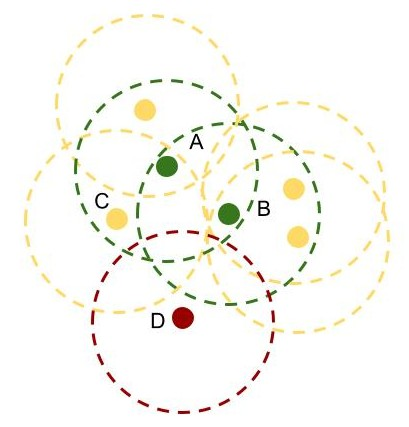
\includegraphics[width=1\textwidth]{figure/dbscan.jpg}
			
			\tiny{Example for DBSCAN, circles display $\epsilon$-neighborhoods, $m = 4$}
			
		\end{center}
	\end{column}
\end{columns}
\begin{itemize}
		\item A new point could be classified as being in-distribution if it lies within a cluster, or out-of-distribution if it lies outside the clusters. 
		\item Disadvantage: Depending on the distance metric $d(\cdot)$, DBSCAN could suffer from the ``curse of dimensionality''. 
		\item Furthermore, the choice of $\epsilon$ and $m$ is not clear a-priori. 
\end{itemize}
	\footnote[frame]{Martin Ester et al. (1996). A density-based algorithm for discovering clusters in large spatial databases with noise. KDD'96: Proceedings of the Second International Conference on Knowledge Discovery and Data Mining. 226–231.}
\end{frame}

\begin{vbframe}{Robustness}
		\begin{itemize}
		\item In general we must differentiate between explanation uncertainty and process uncertainty that lead to non-robust explanations: 
		\begin{enumerate}
			\item Explanation uncertainty tries to answer how an explanation changes if we repeat the experiment. The explanation could differ depending on which subset of data we use for the explanation method and which parameters. 
			\item Process uncertainty tries to answer how an explanation changes if the underlying model is changed. This is interesting since ML models can be non-robust, e.g., because they are trained on noisy data. 
		\end{enumerate}
		\item Here, we focus on the former - explanation uncertainty. We could receive different explanations although we analyse the same model and the same (or a very similar) data point.
	\end{itemize}
\end{vbframe}

\begin{vbframe}{Robustness Measure for LIME and SHAP}  
	\begin{itemize}
		\item One way to quantify the robustness of an explanation is to examine the behavior of the model in a neighborhood of the point of interest. We would like to receive similar explanations for similar inputs. 
		\item In the previous chapter on the limitations of LIME, we already saw an example where LIME produced different explanations for very similar data points (with similar predictions).
		\item For LIME and SHAP, Alvarez-Melis and Jaakkola (2018) derived a notion of stability based on \textbf{locally Lipschitz continuity}: \\
		An explanation method $g:\Xspace \rightarrow \R^m$ is locally Lipschitz if for every $\xv_0 \in \Xspace$ there exist $\delta > 0$ and $\omega \in \R$ such that $||\xv - \xv_0|| < \delta$ implies $||g(\xv) - g(\xv_0)|| < \omega ||\xv - \xv_0||$. \\
		\footnotesize Note that, for LIME, $g$ returns the $m$ coefficients of the surrogate model. \normalsize
		\item According to this definition we can quantify and compare the robustness of explanation models in terms of $\omega$. 
		The closer $\omega$ is to 0, the more robust our explanation method is. 
		\item $\omega$ is rarely known a-priori but it could be estimated as following: 
		$$\hat{\omega}_{X}(\xv) = \underset{x_i \in \mathcal{N}_{\epsilon}(\xv)}{\arg \max} \frac{||g(\xv) - g(\xv_i)||_2}{d(\xv, \xv_i)},$$
		where $\mathcal{N}_{\epsilon}(\xv)$ is the $\epsilon$-neighborhood of $\xv$.
	\end{itemize}
\vspace{2cm}
\footnote[frame]{Alvarez-Melis, D., \& Jaakkola, T. (2018). On the Robustness of Interpretability Methods. ArXiv, abs/1806.08049.}
\end{vbframe}


\begin{comment}
\begin{vbframe}{Sources of Uncertainty}
Two sources of uncertainty could be identified for local explanation methods: 
\begin{itemize}
\item Sampling variance in explaining a single data point. 
E.g., to train a surrogate model for LIME we sample a new data set.   
\item Sensitivity to choice of parameters. E.g., the user needs to determine the sample size and the kernel width to explain a model with LIME. 
\end{itemize}
These sources could lead to different explanations although we analyse the same model and the same (or a very similar) data point. 
\footnote[frame]{Zhang et al. (2019). ``Why Should You Trust My Explanation?'' Understanding Uncertainty in LIME Explanations. arXiv preprint arXiv:1904.12991.} 
\end{vbframe}
\end{comment}


\begin{comment}
\begin{vbframe}{Noisy data}
	\begin{itemize}
		\item What if the ML model was trained on noisy data? Should the explanation model also take up these noisy patterns? 
		\item If we use an explanation model to debug the ML model, it is okay, if our explanation model also takes up the noisy patterns learned in the ML model. 
		\item If we use an explanation model to understand both the predictor but also the underlying true data generating process, we want to focus on the stable patterns learned by the ML model and receive robust explanations. 
	\end{itemize}
\end{vbframe}

\begin{vbframe}{Addtional notes}
	\begin{itemize}
		\item We cannot only impose that the explanation of one particular method is similar for similar data points, but also across multiple IML methods. 
	\end{itemize}
\end{vbframe}

content...
\end{comment}

\endlecture
\end{document}